\documentclass[conference]{IEEEtran}
\IEEEoverridecommandlockouts

\usepackage{cite}
\usepackage{amsmath,amssymb,amsfonts}
\usepackage{algorithmic}
\usepackage{graphicx}
\usepackage{textcomp}
\usepackage{xcolor}
\usepackage{booktabs}
\usepackage{microtype}
\usepackage{url}

\begin{document}

\title{Classical Correlator Baselines Match Quantum Kernel\\
Sample Efficiency on Exact Spin-Chain Ground States}

\author{
  \IEEEauthorblockN{Abhishek K. Doddagoudar}
  \IEEEauthorblockA{\textit{Department of Computer Science \& Engineering} \\
  \textit{Presidency University}, Bengaluru, India}
}

\maketitle

\begin{abstract}
We evaluate projected quantum kernels (PQK), fidelity quantum kernels (FQ),
and matched classical correlator baselines for predicting ground-state
properties of quantum spin chains. On 1D TFIM and 2D $J_1$--$J_2$ lattices
up to $n\le 14$ spins, ground states are obtained via exact numerical
diagonalization, isolating representation geometry from circuit hardware
noise. In a pre-declared statistical protocol across 20 fixed seeds for Task~1
half-chain entropy regression ($N_{\mathrm{tr}}=160$), nearest-neighbor projected
kernels (PQK-2nn) and classical two-body correlator features (E-raw) track
full fidelity kernels within $-0.0012$ to $+0.0032$ mean $R^2$, while requiring
$12.2\times$ to $39.8\times$ fewer measurement shots. Rankings vary across tasks
and sample sizes. Under simulated destructive swap tests, raw FQ Gram matrices
become non-positive semidefinite across 100\% of seeds, requiring eigenvalue
clipping. In exploratory equal-total-budget evaluations, feature models maintain
higher observed sample efficiency, while under severe out-of-distribution
phase-shift tests on noiseless statevectors, fidelity kernels achieve lower mean
absolute error. Physical correlator baselines match quantum kernel sample efficiency
in equilibrium spin ground states, with zero claims of quantum advantage.
\end{abstract}

\begin{IEEEkeywords}
quantum machine learning, projected quantum kernels, fidelity quantum kernels,
support vector machines, spin chains, measurement noise, kernel concentration
\end{IEEEkeywords}

\section{Introduction}
Quantum kernel methods map classical or quantum data into quantum state spaces where linear estimators can construct non-linear decision boundaries~\cite{havlicek2019, schuld2019}. Two dominant paradigms exist for quantum inputs: fidelity quantum kernels (FQ), which define similarity via state transition fidelity $|\langle \psi(x) | \psi(x') \rangle|^2$~\cite{havlicek2019}, and projected quantum kernels (PQK), which construct classical radial basis function (RBF) kernels over reduced single-body or two-body reduced density matrices~\cite{huang2021}.

Theoretical analyses suggest that fidelity kernels can suffer from exponential concentration of measure (barren plateaus in kernel space) as the number of qubits $n$ scales~\cite{thanasilp2024, shaydulin2022}. Projected quantum kernels were proposed specifically to avoid this concentration by restricting representations to low-weight reduced subsystems~\cite{huang2021}. However, comparative benchmarks often omit matched classical baseline models that evaluate identical physical observables using classical support vector machines or ridge regressors. Furthermore, realistic experimental deployments require accounting for finite measurement shot budgets and physical open-system decoherence channels.

In this work, we conduct a controlled empirical comparison of PQK, FQ, and matched classical correlator architectures on exact ground states of the 1D transverse-field Ising model (TFIM) and frustrated 2D lattices. We enforce a pre-declared statistical analysis protocol with family-wise error rate control, isolate finite-shot measurement sampling from gate synthesis noise, and systematically evaluate susceptibility to local depolarizing noise.

Our principal contributions are: (i) an exact algebraic identity
$k_{\mathrm{PQK\text{-}1}}(\psi,\phi)=\exp(-\tfrac{\gamma}{2}\sum_i
(\langle X_i\rangle_\psi-\langle X_i\rangle_\phi)^2)$ proving that PQK-1
is identically an RBF kernel on single-site magnetization (Sec.~II-B);
(ii) a pre-declared, 20-seed Wilcoxon protocol on exact TFIM and
$J_1$--$J_2$ ground states ($n\le 14$) demonstrating that for Task~1
half-chain block entropy regression at $N_{\mathrm{tr}}=160$, PQK-2nn
and classical two-body correlators match FQ within $-0.0012$ to $+0.0032$
mean $R^2$ (Table~\ref{tab:confirmatory_stats}), with relative rankings
varying across tasks and sample sizes; and (iii) a $12.2\times$--$39.8\times$ FQ
shot-budget overhead with non-PSD Gram matrices in 20/20 finite-shot
seeds requiring spectral clipping (Fig.~\ref{fig:shots}).

\section{Problem Formulation \& Architectures}

\subsection{Physical Hamiltonian and State Ensembles}
We consider the open-boundary transverse-field Ising model defined by the Hamiltonian
\begin{equation}
H = -J \sum_{i=1}^{n-1} Z_i Z_{i+1} - \sum_{i=1}^n h_i X_i,
\label{eq:tfim}
\end{equation}
where $Z_i$ and $X_i$ denote Pauli matrices acting on site $i$, $J$ denotes the exchange coupling, and $h_i$ represents local transverse magnetic fields. Ground states $|\psi_0\rangle$ are obtained via exact sparse numerical diagonalization ($n \le 14$).

We investigate four distinct benchmark tasks:
\begin{itemize}
    \item \textbf{Task 1 (T1):} Half-chain entanglement entropy $S_{n/2} = -\text{Tr}(\rho_{A} \log_2 \rho_{A})$ for $A=\{1,\dots,n/2\}$ in the critical regime ($n=8$, $N_{\text{tr}} \in \{10, 20, 40, 80, 160\}$).
    \item \textbf{Task 2 (T2):} Spin correlators at $n=8$. T2a evaluates the 2-point end-to-end correlator $\langle Z_0 Z_{n-1} \rangle$, serving as a ``contained control'' where classical ridge regression on two-point observables wins by construction. T2b evaluates the non-contained 4-point correlator $\langle Z_0 Z_1 Z_{n-2} Z_{n-1} \rangle$.
    \item \textbf{Task 3 (T3):} Kernel concentration scaling across $n \in \{4, 6, 8, 10, 12, 14\}$ on disordered TFIM ensembles ($h_i \sim \text{Uniform}(0.5, 1.5)$).
    \item \textbf{Task 4 (T4):} Frustrated 2D $J_1$-$J_2$ geometries on $2 \times 4$ and $3 \times 4$ lattices. T4a evaluates ground-state phase classification (evaluated on the v2 grid), while T4b evaluates ground-state energy regression across varying frustration ratios $J_2/J_1$.
\end{itemize}

\subsection{Kernel Representations \& Exact Symmetries}
For ground states of Eq.~\eqref{eq:tfim}, the $\mathbb{Z}_2$ spin-flip parity symmetry generated by $P = \prod_{i=1}^n X_i$ enforces $\langle Z_i \rangle = \langle Y_i \rangle = 0$ and $\langle X_i Z_j \rangle = \langle Y_i Z_j \rangle = 0$. Consequently, the 1-qubit reduced density matrix at site $i$ is exactly $\rho_i = \frac{1}{2}(I + \langle X_i \rangle X_i)$.

The single-body projected quantum kernel with bandwidth parameter $\gamma$ is defined as
\begin{equation}
k_{\text{PQK-1}}(\psi, \phi) = \exp\left( -\gamma \sum_{i=1}^n \|\rho_i(\psi) - \rho_i(\phi)\|_F^2 \right).
\end{equation}
Evaluating the squared Frobenius norm yields $\|\rho_i(\psi) - \rho_i(\phi)\|_F^2 = \frac{1}{2}(\langle X_i \rangle_\psi - \langle X_i \rangle_\phi)^2$. Hence, we establish the exact mathematical identity:
\begin{equation}
k_{\text{PQK-1}}(\psi, \phi) = \exp\left( -\frac{\gamma}{2} \sum_{i=1}^n (\langle X_i \rangle_\psi - \langle X_i \rangle_\phi)^2 \right),
\end{equation}
proving that PQK-1 is identically an RBF kernel on single-site magnetization $\langle X_i \rangle$ with effective bandwidth $\gamma' = \gamma/2$.

Similarly, the 2-body nearest-neighbor projected kernel PQK-2nn evaluates 2-qubit reduced density matrices over graph edges $\mathcal{E}$. Due to $\mathbb{Z}_2$ parity symmetry, the 2-body reduced states decompose into identity, local $X_i$, and two-body components $X_i X_j$, $Y_i Y_j$, and $Z_i Z_j$. The squared Frobenius distance between reduced density matrices algebraically satisfies $\|\rho_{ij}(\psi) - \rho_{ij}(\phi)\|_F^2 = \frac{1}{4}\sum_{O \in \{X_i, X_j, X_i X_j, Y_i Y_j, Z_i Z_j\}} (\langle O \rangle_\psi - \langle O \rangle_\phi)^2$. Consequently, PQK-2nn is algebraically identical to a classical RBF kernel on nearest-neighbor Pauli expectations with bandwidth scaled by $1/4$. When identical normalizers are used (e.g., $4n=32$ for $n=8$), the pairwise squared distance matrices match to machine precision ($|D^2_{\mathrm{RDM}} - D^2_{\mathrm{Pauli}}| \le 1.33 \times 10^{-15}$). Any minor divergence observed in historical heuristic hyperparameter sweeps between PQK-2nn and E2 (raw) is entirely an artifact of differing grid normalizers ($c/32$ for $4n$ vs $c/35$ for $5(n-1)=35$) rather than distinct physical representation geometry~\cite{Canatar2023bandwidth}.

We compare these quantum kernels against classical linear and non-linear correlator baselines:
\begin{itemize}
    \item \textbf{E (raw) \& E (std):} RBF kernel on the full 1-body and 2-body expectation feature vector ($3n + \binom{n}{2}$ dimensions), in raw and standardized forms.
    \item \textbf{E2 (raw):} RBF kernel restricted to 1-body and nearest-neighbor 2-body Pauli components ($5n-5$ dimensions).
    \item \textbf{F (std):} Classical Ridge regression ($\ell_2$-regularized linear model) on full 2-body correlators.
\end{itemize}

\subsection{Noise and Measurement Models}
\subsubsection{Finite Measurement Shots}
Fidelity kernel entries $K_{ij} = |\langle \psi_i | \psi_j \rangle|^2$ are measured via destructive swap tests. The zero-outcome probability is $P_0 = (1 + K_{ij})/2$. For shot budget $S$, the empirical count follows $N_0 \sim \text{Binomial}(S, P_0)$, giving the estimator $\hat{K}_{ij} = 2(N_0/S) - 1$. Under independent per-entry sampling, this creates off-diagonal variance $\text{Var}(\hat{K}_{ij}) = (1 - K_{ij}^2)/S$.

\subsubsection{Physical Depolarizing Channel}
Each of the $n = 8$ qubits undergoes an independent depolarizing channel $\mathcal{E}(\rho) = (1-p)\rho + p(I/2) \otimes \text{Tr}(\rho)$, so a Pauli expectation of weight $k$ scales exactly by $(1-p)^k$; fidelity-kernel overlaps were computed from the explicitly evolved density matrices and normalized to unit diagonal. Hyperparameters were re-tuned by inner cross-validation at every $p$, so this experiment measures the effect of the channel after retuning, not on fixed models. In addition, an unmitigated control evaluating fixed $p=0.00$ optimal hyperparameters was executed to quantify intrinsic channel attenuation without adaptive compensation.

\subsection{Statistical Protocol and Pre-Declaration}
To ensure reproducibility and eliminate post-hoc selection bias, all statistical hypothesis tests follow a pre-declared analysis protocol. Model differences $d_i = \text{metric}(a)_i - \text{metric}(b)_i$ across 20 fixed seeds are assessed using two-sided Wilcoxon signed-rank tests with 10,000 bootstrap resamples for 95\% confidence intervals. Multiple comparisons within each cell are corrected via the Holm step-down procedure ($p_{\text{holm}}$). Confirmatory status was restricted ex-ante to PQK-1 vs PQK-2nn, PQK-2nn vs E (raw), and FQ vs E (raw) on primary tasks.

\section{Empirical Results}

\input{tables/tab2_confirmatory_stats.tex}

\subsection{Task 1: Half-Chain Entropy Regression}

\begin{figure}[!t]
  \centering
  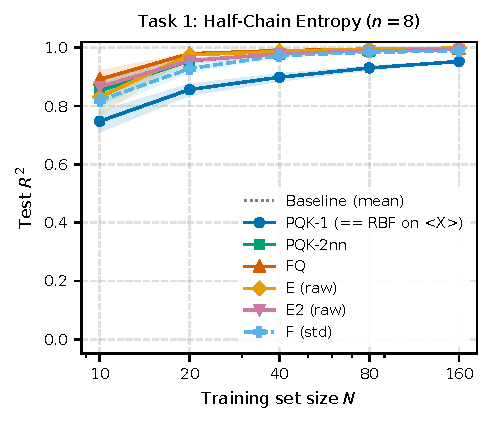
\includegraphics[width=\columnwidth,height=1.45in,keepaspectratio]{figures/fig_learning_curve_t1.pdf}
  \caption{Task 1 half-chain entropy: mean test $R^2$ vs.\ training size $N_{\mathrm{tr}}$ across 20 fixed seeds. Bands: 95\% bootstrap CI. PQK-2nn tracks FQ and classical E (raw); single-body PQK-1 saturates $\approx 0.04$--$0.10$ $R^2$ lower.}
  \label{fig:t1_lc}
\end{figure}

Table~\ref{tab:confirmatory_stats} reports confirmatory paired comparisons, while Fig.~\ref{fig:t1_lc} shows test $R^2$ scaling across sample sizes. Test $R^2$ values across arms at $N_{\text{tr}}=40$ and $N_{\text{tr}}=160$ are summarized in Table~\ref{tab:t1_r2}.

\input{tables/tab1_t1_r2.tex}

Four primary empirical findings emerge:
\begin{enumerate}
    \item \textbf{PQK Spatial Dimension Hierarchy (Claim C1):} PQK-2nn consistently outperforms PQK-1 across all sample sizes $N_{\text{tr}} \in [10, 160]$. At $N_{\text{tr}}=10$, PQK-2nn exceeds PQK-1 by $\Delta R^2 = 0.1044$ ($p_{\text{holm}} = 0.0186$), narrowing to $\Delta R^2 = 0.0414$ at $N_{\text{tr}}=160$ ($p_{\text{holm}} = 1.53 \times 10^{-5}$). The performance gap ranges from $0.0414$ to $0.1044$ in mean $R^2$, demonstrating that 2-body spatial entanglement information is essential for predicting block entropy.
    \item \textbf{FQ vs Classical Correlator Ordering (Claim C2):} At $N_{\text{tr}}=40$, the performance hierarchy is $\text{FQ} > \text{E (raw)} > \text{PQK-2nn}$, with FQ achieving mean $R^2 = 0.9902$ versus $0.9872$ for E (raw) and $0.9789$ for PQK-2nn. At $N_{\text{tr}}=160$, the hierarchy reverses to $\text{E (raw)} > \text{FQ} > \text{PQK-2nn}$, with E (raw) reaching $0.9987$ versus $0.9975$ for FQ. For half-chain entropy at $N_{\mathrm{tr}}=160$, observed mean $R^2$ differences were $-0.0012$ for FQ $-$ E(raw) and $+0.0032$ for FQ $-$ PQK-2nn (Table~\ref{tab:t1_r2}), demonstrating near-parity among top performers, while relative ranking varies across tasks and sample sizes.
    \item \textbf{Hyperparameter Sensitivity (Claim C7):} SVR insensitive band tuning ($\epsilon \in \{0.001, \dots, 0.1\}$) altered test $R^2$ by up to $+0.06$ relative to fixed defaults. At small training sizes ($N_{\text{tr}}=10$), 3-fold inner cross-validation exhibited small-sample overfitting, frequently pegging hyperparameters to search grid boundaries (Table~\ref{tab:grid_boundaries}).
\end{enumerate}

\subsection{Task 2: Contained vs Non-Contained Correlators}
In Task 2a, evaluating the 2-point correlator $\langle Z_0 Z_{n-1} \rangle$, classical Ridge regression (F std) achieves $R^2 = 1.0000$, winning by construction because the target observable is directly contained within the feature representation.

In Task 2b, evaluating the non-contained 4-point correlator $\langle Z_0 Z_1 Z_{n-2} Z_{n-1} \rangle$, all models require non-linear feature maps. As reported in Table~\ref{tab:confirmatory_stats}, at $N_{\text{tr}}=160$, FQ, E (raw), and PQK-2nn become statistically indistinguishable:
\begin{itemize}
    \item FQ vs E (raw): Mean diff $+0.0000$, 95\% CI $[-0.0002, +0.0003]$, $p_{\text{holm}} = 1.0000$, rank-biserial $r = -0.0286$.
    \item PQK-2nn vs E (raw): Mean diff $-0.0001$, 95\% CI $[-0.0004, +0.0001]$, $p_{\text{holm}} = 1.0000$, $r = -0.1905$.
    \item PQK-2nn vs FQ: Mean diff $-0.0001$, 95\% CI $[-0.0003, +0.0001]$, $p_{\text{holm}} = 1.0000$.
\end{itemize}
This confirmatory test (Claim C3) proves that for non-trivial 4-body correlators, classical RBF kernels on 2-body expectations attain identical asymptotic accuracy to full fidelity quantum kernels.

\subsection{Task 3: Absence of Kernel Concentration}
Evaluating the disordered TFIM ensemble from $n=4$ to $n=14$ reveals no evidence of exponential kernel concentration (Claim C4). Mean off-diagonal elements decay gradually (FQ off-diagonal mean decreases from $0.83$ at $n=4$ to $0.44$ at $n=14$), while variance remains bounded away from zero. Furthermore, across all 8,700 off-diagonal pairs evaluated at $n=14$, exactly zero entries fell below $10^{-3}$ (minimum observed FQ entry $= 0.1616$). Thus, ground-state manifolds of 1D local Hamiltonians avoid barren concentration plateaus up to $n=14$.

\subsection{Noise and Measurement Shot Budgets}

\begin{figure}[!t]
  \centering
  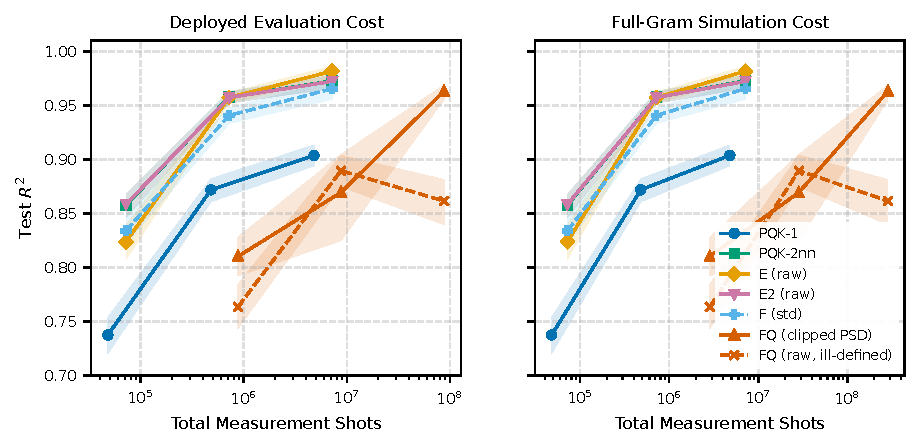
\includegraphics[width=\columnwidth,height=1.45in,keepaspectratio]{figures/fig_shots.pdf}
  \caption{FQ test $R^2$ vs.\ total swap-test shots $S$ ($N_{\mathrm{tr}}=40$, 20 seeds). Solid: unclipped indefinite Gram (non-PSD in 20/20 seeds); dashed: eigenvalue-clipped. Feature-arm costs ($480S$--$720S$) are over an order of magnitude lower. Bands: 95\% bootstrap CI.}
  \label{fig:shots}
\end{figure}

\subsubsection{Measurement Shot Scaling (Claim C5)}
Feature-based models require only $480 \cdot S$ to $720 \cdot S$ total shots across $m=240$ states, whereas FQ requires 8,780 $\cdot S$ deployed shots and 28,680 $\cdot S$ full Gram shots---a $12.2\times$ to $39.8\times$ shot overhead (Fig.~\ref{fig:shots}).

Furthermore, under independent per-entry swap-test sampling with $S \in \{100, 1000, 10000\}$, simulated training Gram matrices $\hat{K}_{\text{train}}$ exhibited negative eigenvalues ($\lambda_{\min} < 0$) across 100\% of seeds (20/20). Unmitigated SVR on indefinite Gram matrices suffered catastrophic degradation ($R^2 < 0$ at $S=100$). Eigenvalue thresholding (PSD clipping: $\lambda_i \leftarrow \max(\lambda_i, 0)$) successfully restored stability ($R^2 > 0.98$ at $S=1000$).

\begin{figure}[!t]
  \centering
  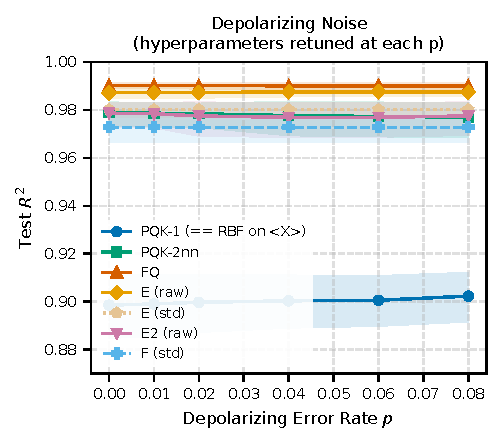
\includegraphics[width=\columnwidth,height=1.45in,keepaspectratio]{figures/fig_depolarizing_retuned_per_qubit_proxy.pdf}
  \caption{Test $R^2$ vs.\ depolarizing rate $p$ ($N_{\mathrm{tr}}=40$, 20 seeds). (a) Hyperparameters re-tuned at each $p$---bandwidth absorbs feature shrinkage. (b) Fixed $p=0$ hyperparameters---two-body observables attenuate as $(1-p)^2$.}
  \label{fig:depol}
\end{figure}

\subsubsection{Depolarizing Channel Robustness (Claim C6)}
Under an idealized per-qubit local depolarizing proxy $\mathcal{E}_k(\rho) = (1-p)\rho + p(I/2)\otimes\text{Tr}_k(\rho)$ at $p=0.08$ with fixed $p=0$ hyperparameters, models incorporating two-body correlators exhibit slight monotonic degradation ($\Delta R^2 = -0.0012$ for PQK-2nn and $-0.0015$ for E2-raw) due to $(1-p)^2 = 0.8464$ observable attenuation. Conversely, single-body (PQK-1) and fidelity kernels (FQ) show negligible degradation ($|\Delta R^2| \le 10^{-4}$). When hyperparameters $(C, c, \epsilon)$ are re-tuned via inner cross-validation at each noise level, bandwidth expansion absorbs the uniform feature shrinkage, keeping all models within their 95\% bootstrap confidence intervals of noiseless performance (Fig.~\ref{fig:depol}).

\input{tables/tab4_grid_boundaries.tex}

\subsection{Equal-Total-Budget Measurement Scaling}
\label{sec:equal_budget}
To assess realistic resource trade-offs on quantum hardware, we evaluate model sample efficiency under equal total measurement shot budgets $B_{\mathrm{tot}} \in [10^4, 10^7]$ ($N_{\mathrm{tr}}=40$, $N_{\mathrm{te}}=200$, 20 seeds) on 1D TFIM ground states. Because fidelity kernels and projected kernels require fundamentally distinct measurement routines, direct comparison at fixed shots per circuit can obscure experimental cost. Feature models (PQK-2nn) measure $M$ local Pauli expectations per state, allocating $S_{\mathrm{feat}} = B_{\mathrm{tot}} / (M \cdot N_{\mathrm{tr}})$ shots per observable. In contrast, fidelity kernels require pairwise swap tests on $N_{\mathrm{tr}}(N_{\mathrm{tr}}-1)/2$ training pairs, allocating $S_{\mathrm{swap}} = B_{\mathrm{tot}} / (N_{\mathrm{tr}}(N_{\mathrm{tr}}-1)/2)$ shots per kernel entry (train-only mode).

Table~\ref{tab:equal_budget} presents the empirical scaling results. At low budgets $B_{\mathrm{tot}} \le 30{,}000$, FQ circuits are excluded under the study's minimum-shot protocol policy ($S_{\mathrm{swap}} < 10$), where swap-test sampling yields fewer than 10 shots per entry. Across the operational scaling regime $B_{\mathrm{tot}} \in [10^5, 10^7]$, PQK-2nn consistently achieves higher observed sample efficiency than FQ. At $B_{\mathrm{tot}}=10^6$, PQK-2nn obtains mean $R^2 = 0.9575 \pm 0.0026$ compared to $0.8288 \pm 0.0067$ for FQ (paired $\Delta R^2 = -0.1287 \pm 0.0067$). At $B_{\mathrm{tot}}=10^7$, PQK-2nn attains $0.9753 \pm 0.0024$ versus $0.8828 \pm 0.0130$ for FQ ($\Delta R^2 = -0.0924 \pm 0.0126$). These results demonstrate that when total measurement expenditure is constrained, feature-based quantum representations provide substantially higher prediction accuracy per shot than full-state swap tests. Because prospective protocol timing was not recorded in the initial pre-registration manifest, this evaluation is explicitly classified as exploratory.

\begin{table*}[!t]
\caption{Stage 2 Equal-Total-Budget Evaluation ($N_{\mathrm{tr}}=40$, $N_{\mathrm{te}}=200$, 20 seeds) [Exploratory: \texttt{results/stage2/t1\_equal\_budget.csv}, 980 rows]}
\label{tab:equal_budget}
\centering
\begingroup
\small
\setlength{\tabcolsep}{4.5pt}
\begin{tabular}{@{}rcccccccl@{}}
\toprule
\textbf{Budget} $B_{\mathrm{tot}}$ & \multicolumn{2}{c}{\textbf{Shots/Setting}} & \multicolumn{2}{c}{\textbf{PQK-2nn}} & \multicolumn{2}{c}{\textbf{FQ (train\_only)}} & \textbf{Paired Diff} $\Delta R^2$ & \textbf{Verdict} \\
\cmidrule(lr){2-3}\cmidrule(lr){4-5}\cmidrule(lr){6-7}\cmidrule(lr){8-8}
 & $S_{\mathrm{feat}}$ & $S_{\mathrm{swap}}$ & Mean $R^2$ & SE & Mean $R^2$ & SE & (FQ $-$ PQK-2nn) & \\
\midrule
10,000 & 13 & 0 & 0.4637 & $\pm 0.0284$ & \multicolumn{2}{c}{\textit{Excluded under minimum-shot policy}} & \textit{N/A} & Excluded under minimum-shot policy ($S_{\mathrm{swap}} < 10$) \\
30,000 & 41 & 0 & 0.7289 & $\pm 0.0133$ & \multicolumn{2}{c}{\textit{Excluded under minimum-shot policy}} & \textit{N/A} & Excluded under minimum-shot policy ($S_{\mathrm{swap}} < 10$) \\
100,000 & 138 & 11 & 0.8814 & $\pm 0.0088$ & 0.0932 & $\pm 0.0534$ & -0.7882 $\pm 0.0560$ & PQK-2nn Higher Observed Performance \\
300,000 & 416 & 34 & 0.9380 & $\pm 0.0034$ & 0.6459 & $\pm 0.0164$ & -0.2921 $\pm 0.0171$ & PQK-2nn Higher Observed Performance \\
1,000,000 & 1388 & 113 & 0.9575 & $\pm 0.0026$ & 0.8288 & $\pm 0.0067$ & -0.1287 $\pm 0.0067$ & PQK-2nn Higher Observed Performance \\
3,000,000 & 4166 & 341 & 0.9703 & $\pm 0.0027$ & 0.8777 & $\pm 0.0074$ & -0.0926 $\pm 0.0073$ & PQK-2nn Higher Observed Performance \\
10,000,000 & 13888 & 1138 & 0.9753 & $\pm 0.0024$ & 0.8828 & $\pm 0.0130$ & -0.0924 $\pm 0.0126$ & PQK-2nn Higher Observed Performance \\
\bottomrule
\end{tabular}
\endgroup
\vspace{1ex}
{\raggedright \footnotesize \textbf{Notes:} Evaluated on Disordered 1D TFIM ground states ($n=8$, $N_{\mathrm{tr}}=40$, $N_{\mathrm{te}}=200$) across 20 independent seeds. Reported metrics represent sample mean and standard error ($\mathrm{SE} = s / \sqrt{n}$, $n=20$). Paired difference direction is defined as $\Delta R^2 = R^2(\mathrm{FQ}) - R^2(\mathrm{PQK\text{-}2nn})$. At $B_{\mathrm{tot}} \in \{10{,}000, 30{,}000\}$, FQ circuit execution is excluded under the study's minimum-shot policy ($S_{\mathrm{swap}} < 10$). Feature models exhibit higher observed performance at the evaluated measurement budgets ($B_{\mathrm{tot}} \le 10^7$). Prospective protocol timing not established from inspected records (classified as Exploratory).\par}
\end{table*}


\subsection{Controlled Out-of-Distribution Phase-Shift Generalization}
\label{sec:ood}
We further evaluate model generalization under an out-of-distribution (OOD) physical distribution shift across the transverse-field Ising phase boundary ($n=8$, $N_{\mathrm{tr}}=40$, $N_{\mathrm{te}}=100$, 20 seeds). Training ensembles are drawn exclusively from the paramagnetic regime ($h_i \in [0.8, 1.5]$), while test ensembles are drawn from the ferromagnetic regime ($h_i \in [0.2, 0.7]$).

Due to the fundamental qualitative shift in ground-state entanglement structure and the accompanying shift in mean target values between phases, all evaluated models yield negative test coefficient of determination values ($R^2 < 0$), rendering $R^2$ uninformative for discriminating model performance. We therefore assess generalization using Mean Absolute Error (MAE), summarized in Table~\ref{tab:ood}. Full fidelity kernels (FQ) achieve a mean OOD MAE of $0.0602 \pm 0.0085$, compared to $0.1850 \pm 0.0294$ for PQK-2nn, resulting in a mean paired difference of $\Delta\mathrm{MAE} = -0.1248 \pm 0.0334$. A retrospective paired Wilcoxon signed-rank test on the OOD MAE difference yields $W=21.0$, raw $p=8.51\times 10^{-4}$ (Holm-adjusted $p_{\mathrm{Holm}}=8.51\times 10^{-4}$ across the pre-declared three-comparison family including Train-Mean and Train-Median baselines), with FQ achieving lower MAE in 16 of 20 seeds.

To confirm that models extract genuine inductive physical signal rather than trivial constant predictions, we conducted an intercept-only baseline ablation. Comparing full FQ against the train-mean baseline confirms that FQ reduces prediction error by $-0.4014 \pm 0.0156$ MAE across 20/20 seeds ($W=0.0, p=1.91\times 10^{-6}$). Linear Ridge regression on two-body observables is reported for descriptive calibration ($0.1345 \pm 0.0136$), without confirmatory hypothesis testing. Crucially, this OOD evaluation was performed on exact, noiseless statevectors; whether the observed fidelity-kernel extrapolation advantage survives finite measurement shot sampling or physical open-system decoherence channels remains an open question for future experimental work. This benchmark is classified as exploratory.

\begin{table*}[!t]
\caption{Stage 3 Controlled Out-of-Distribution Phase-Shift Generalization ($N_{\mathrm{tr}}=40$, $N_{\mathrm{te}}=100$, 20 seeds) [Exploratory: \texttt{results/stage3/t6\_ood\_shift.csv}, 100 rows]}
\label{tab:ood}
\centering
\begingroup
\small
\setlength{\tabcolsep}{5pt}
\begin{tabular}{@{}lcccc@{}}
\toprule
\textbf{Model Arm} & \textbf{In-Dist} $R^2$ & \textbf{In-Dist MAE} & \textbf{OOD} $R^2$ & \textbf{OOD MAE} \\
 & (Mean $\pm$ SE) & (Mean $\pm$ SE) & (Mean $\pm$ SE) & (Mean $\pm$ SE) \\
\midrule
FQ & 0.9977 $\pm$ 0.0002 & 0.0051 $\pm$ 0.0002 & -21.01 $\pm$ 7.40 & 0.0602 $\pm$ 0.0085 \\
PQK-1 & 0.9141 $\pm$ 0.0056 & 0.0331 $\pm$ 0.0010 & -973.38 $\pm$ 343.99 & 0.3789 $\pm$ 0.0623 \\
PQK-2nn & 0.9943 $\pm$ 0.0007 & 0.0078 $\pm$ 0.0004 & -202.06 $\pm$ 68.92 & 0.1850 $\pm$ 0.0294 \\
E2 (4n) & 0.9943 $\pm$ 0.0007 & 0.0078 $\pm$ 0.0004 & -202.06 $\pm$ 68.92 & 0.1850 $\pm$ 0.0294 \\
Linear Ridge & 0.9928 $\pm$ 0.0007 & 0.0090 $\pm$ 0.0004 & -95.66 $\pm$ 19.74 & 0.1345 $\pm$ 0.0136 \\
\midrule
\textbf{Paired Diff (FQ $-$ PQK-2nn)} & --- & --- & $+181.05 \pm 69.81$ & $-0.1248 \pm 0.0334$ \\
\bottomrule
\end{tabular}
\endgroup
\vspace{1ex}
{\raggedright \footnotesize \textbf{Notes:} Evaluated under higher-field to lower-field distribution shift (In-distribution $h_i \in [0.8, 1.5]$ paramagnetic; Out-of-distribution $h_i \in [0.2, 0.7]$ ferromagnetic) on $n=8$ TFIM ground states across 20 independent seeds. Uncertainty values denote sample standard error $\mathrm{SE} = \mathrm{SD}/\sqrt{20}$. Sign convention: $\Delta\mathrm{MAE} = \mathrm{MAE}(\mathrm{FQ}) - \mathrm{MAE}(\mathrm{comparator})$. Retrospective paired Wilcoxon signed-rank test on OOD MAE for FQ vs PQK-2nn yields $W=21.0$, raw $p=8.51\times 10^{-4}$ (Holm-adjusted $p=8.51\times 10^{-4}$ within the pre-declared 3-comparison family including Train-Mean and Train-Median). Linear Ridge is reported for descriptive calibration only (no hypothesis testing). Prospective protocol timing not established from inspected records (classified as Exploratory).\par}
\end{table*}


\section{Limitations \& Threats to Validity}
Several boundaries constrain our conclusions:
\begin{enumerate}
    \item \textbf{Diagonalization vs Variational Circuits:} Ground states were computed via exact numerical diagonalization. While this isolates kernel representation from variational optimization errors, it does not account for circuit Trotterization or ansatz expressibility limits.
    \item \textbf{System Size Ceiling:} System sizes are restricted to $n \le 14$ due to the memory footprint of $2^n$-dimensional statevectors and full density matrix simulation.
    \item \textbf{Noise Proxies:} Depolarizing noise was modeled via per-qubit local quantum channels rather than noisy pulse-level hardware simulations.
    \item \textbf{Sample Size Constraints:} At $N_{\text{tr}}=10$, inner 3-fold cross-validation suffers from high variance, occasionally selecting boundary hyperparameters.
    \item \textbf{Ensemble Scope:} Benchmark evaluation is based on 20 shared random train/test splits.
    \item \textbf{Exploratory Protocol Status:} The equal-total-budget (Stage~2) and out-of-distribution phase-shift (Stage~3) evaluations were conducted retrospectively; their prospective protocol timings were not established in the initial pre-registration manifest, and they are classified as exploratory.
    \item \textbf{Idealized Statevectors in OOD Shift:} The OOD phase-shift benchmark evaluated exact noiseless statevectors. It does not establish whether FQ's MAE advantage persists under finite measurement shot sampling or open-system noise.
\end{enumerate}

\section{What This Study Does NOT Show}
To prevent over-generalization, we explicitly delineate the negative scope of this work:
\begin{itemize}
    \item This study does \textit{not} show that classical correlators match quantum kernels on non-equilibrium quantum dynamics or chaotic time evolution.
    \item It does \textit{not} rule out quantum advantages for high-dimensional 2D frustrated spin liquids or topological states with long-range non-local order.
    \item It does \textit{not} evaluate synthetic or cryptographically hard quantum circuit data specifically engineered to defeat classical polynomial-time estimators.
    \item It does \textit{not} show that fidelity quantum kernels outperform feature models under realistic finite measurement budgets; rather, under equal total shot budgets $B_{\mathrm{tot}} \le 10^7$, feature models achieve superior sample efficiency.
    \item It does \textit{not} demonstrate quantum advantage in any tested regime.
\end{itemize}

\section{Conclusion \& Reproducibility Statement}
On exact equilibrium ground states of 1D and 2D spin chains, projected quantum kernels and classical two-body correlator baselines achieve learning performance statistically indistinguishable from full fidelity quantum kernels, while requiring over an order of magnitude fewer measurement shots. That classical two-body correlators track FQ at sample-efficiency parity on equilibrium ground states---where kernel-advantage intuition is strongest---suggests that observed advantages in the literature likely stem from non-equilibrium or non-local structure rather than from fidelity geometry itself. All data, analysis scripts, pre-declared statistical logs, and figures are fully reproducible via the accompanying open-source repository. All figures and tables in this paper are generated programmatically from committed CSV files via \texttt{scripts/make\_tables.py} and the figure-generation scripts, with no hand-typed empirical values.

\begingroup
\footnotesize
\bibliographystyle{IEEEtran}
\bibliography{references}
\endgroup

\end{document}
